\setAuthor{Mihkel Kree}
\setRound{piirkonnavoor}
\setYear{2008}
\setNumber{G 9}
\setDifficulty{8}
\setTopic{Dünaamika}

\prob{Plokid}
Polüspast ehk liitplokk koosneb seitsmest plokist (vt. joonist). Koormiste massid $M$ ja $\gamma M$ on näidatud joonisel. Missuguse kiirendusega hakkavad liikuma äärmised koormised? Mis tingimust peab rahuldama suurus $\gamma$, et äärmised koormised hakkaksid langema? Plokkide ja nööri mass jätta arvestamata ning nöör lugeda venimatuks. 

\begin{center}
	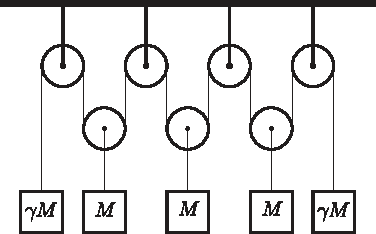
\includegraphics[width=0.6\linewidth]{2008-v2g-09-yl}
\end{center}

\hint
Ülesandes on kolm tundmatut: keskmiste plokkide kiirendused, äärmiste plokkide kiirendused ning niidi pinge. Vastavate tundmatute leidmiseks on vaja kolme võrrandit: kaks tulenevad Newtoni II seadusest ning üks tuleb niidi venimatuse tingimusest.

\solu
Rakendades Newtoni II seadust näeme, et kõik kolm keskmist koormist hakkavad liikuma võrdse kiirendusega $a_0$: 
\[
M a_0 = 2T - Mg,
\]
kus $T$ on niidi pinge. Rakendades Newtoni II seaduste äärmiste koormiste jaoks saame
\[
\gamma M a_1 = T - \gamma Mg,
\]
kus $a_1$ on äärmiste koormiste kiirendus. Elimineerides niidi pinge $T$ saame
\[
2\gamma a_1 - a_0 = g - 2\gamma g.
\] 
Nööri venimatus avaldub kujul $a_1 = -3a_0$, millest tulenevalt 
\[
-2 \gamma a_{1}-\frac{a_{1}}{3}=(2 \gamma-1) g \quad \Rightarrow \quad a_{1}=\frac{1-2 \gamma}{2 \gamma+1 / 3} g.
\]
Äärmised koormised hakkavad langema, kui $a_1$ on negatiivne. Selle jaoks peab kehtima
\[
1-2 \gamma<0 \quad\Rightarrow\quad \gamma>\frac{1}{2}.
\]
\probend